\section{A Sub-Quadratic Algorithm for the \texorpdfstring{$k$}{}-SP and \texorpdfstring{$k$}{}-SPI Problems}\label{sec:k-seq}
In this section, we describe an algorithm that, given a sequence $\requests$ of $n$ requests in $2$-dimensions, computes the optimal solution to the $k$-SP and $k$-SPI problems in $\tilde{O}(n^{1.8}\Phi(n)\log(n\Delta))$ time. We begin by describing our algorithm for the $k$-SP problem and discuss how it can be extended to the $k$-SPI problem in Section~\ref{sec:kspi-extension-sub}.


\subsection{Algorithm for the \texorpdfstring{$k$}{}-SP Problem}
Initialize $\mcC$ to the leaf cells of $\mcH$. Let $M^{\mcC}=(M, B^{\mcC})$ be the extended matching maintained by the algorithm and initialized to $M=\emptyset$ and $B^{\mcC}=\emptyset$. For each point $v \in A\cup B$, let $y(v)$ denote its dual weight initialized to $y(v)=0$. Let $B_F$, initialized to $B$, be the free points of $B$ with respect to $M^{\mcC}$. For each cell $\cell$ that contains at least one free point $b \in B_F$, let $P_\cell$ denote the minimum net-cost augmenting path inside $\cell$. Initially, since $\cell$ is a leaf of $\mcH$, it contains only one point $b \in B_F$, and therefore, $P_{\cell}$ is this point with a net-cost equal to $\distance{b}{\mcC}$. Our algorithm maintains a priority queue $\pq$ storing every leaf cell $\cell\in\mcC$ with at least one free vertex with a key of $\phi(P_\cell)$. 
At any time during the execution of our algorithm, let $\cell_{\min}$ be the cell with the smallest key in $\pq$ and let $\ymax$ be the key of $\cell_{\min}$.
Execute the following steps until $\pq$ becomes empty:

\begin{itemize}
    \item While $|B_F| > k$, 
    \begin{itemize}
        \item {\it Extended Hungarian search step:} Extract the cell $\cell$ with the minimum key of $\ymax$ from $\pq$. Augment the matching $M^\mcC$ along $P_\cell$ and update the key of $\cell$ in $\pq$ (See Section~\ref{subsubsec:global} for details).
    \end{itemize}
    \item {\it Merge step:} If $\mcC=\{\cell^*\}$, remove $\cell^*$ from $\pq$ and return the matching $M$ of $M^{\mcC}$. Otherwise, pick a cell $\cell'\in\mcC$ with the smallest perimeter and let $\cell$ and $\cell''$ be the parent and sibling of $\cell'$ in $\mcH$, respectively. Erase the divider of $\cell$, i.e., set $\mcC=\mcC\setminus\{\cell',\cell''\}\cup \{\cell\}$. 
    We execute a Merge procedure that updates the matching $M^\mcC$ inside the cell $\cell$ so that $\phi(P_\cell)$ is at least $\ymax$ (See Section~\ref{subsubsec:local} for details). At this point, the size of the updated extended matching $M^{\mcC}$ may not be $(n-k)$, i.e., there may be more than $k$ free points.
\end{itemize}

\paragraph{Invariants.} For each cell $\cell \in \mcC$, let $y_\cell= \max_{b\in B_\cell}y(b)$. During the execution of our algorithm,
\begin{itemize}
    \item[(I1)] the extended matching $M^\mcC, y(\cdot)$ is feasible,
    \item[(I2)] For each cell $\cell \in \mcC$, $y_\cell \le \ymax$ and for all free point $b\in B_\cell$, $y(b)=y_{\cell}$, and,
   \item[(I3)] The $\ymax$-value is non-decreasing. Furthermore, after each step of the algorithm, $\ymax$ denotes the smallest net-cost of all augmenting paths with respect to $M^{\mcC}$.
\end{itemize}


\subsubsection{Details of the Extended Hungarian Search Step}\label{subsubsec:global} 
Given a feasible extended matching $M^\mcC, y(\cdot)$  and a cell $\cell\in\mcC$, the extended Hungarian search procedure computes the minimum net-cost augmenting path $P_\cell$ and augments $M^\mcC$ along $P_\cell$. It then computes the new minimum net-cost augmenting path and updates the key of $\cell$ in $\pq$ to be its net-cost. 
This procedure is similar to the classical Hungarian search procedure executed on $\mcG_\cell$ and is mildly modified to include the augmenting paths that end at the boundary of $\cell$. 
Details of the procedure are as follows. 
\begin{enumerate}
\item {\it Update duals:} With $s$ as the source vertex, execute Dijkstra's shortest path algorithm on the residual graph $\mcG_\cell$. Let $P_v$ be the shortest path from $s$ to each $v\in A_\cell\cup B_\cell$ and let $\kappa_v$ be the cost of $P_v$. Let
\begin{equation}\label{eq:global-kappa}
    \kappa = \min\{ \min_{a\in \freeofcell{A}{\cell}}\kappa_a, \min_{b\in B_\cell}\kappa_b + s(b)\}.
\end{equation}
For any $v \in A_\cell\cup B_\cell$, if $\kappa_v < \kappa$, set $ y(v) \leftarrow y(v) +\kappa - \kappa_v$.
\item {\it Augment:} Let $u\in \freeofcell{A}{\cell}\cup B_\cell$ be the point realizing the minimum distance in Equation~\eqref{eq:global-kappa}. Let $P$ be the augmenting path obtained by removing $s$. Augment $M^\mcC$ along $P$. 
\item {\it Update key:} If $B_\cell$ has no free points, then remove $\cell$ from $\pq$. Otherwise,
\begin{enumerate}
    \item Recompute the residual graph $\mcG_{\cell}$ with respect to the updated matching,
    \item With $s$ as the source, execute the Dijkstra's shortest path algorithm on $\mcG_\cell$. For each $v \in A_\cell\cup B_\cell$, let $\kappa_v$ be the distance from $s$ to $v$.
    \item  Update the key of $\cell$ in $\pq$ to $\kappa_\cell = \min\{ \min_{a\in \freeofcell{A}{\cell}}\kappa_a, \min_{b\in B_\cell}\kappa_b + s(b)\}$.
\end{enumerate}   
\end{enumerate}
% \vspace{0.2em}

Lemma~\ref{lemma:hung_properties} establishes the properties of the extended Hungarian search procedure.
\begin{restatable}{lemma}{hungarianProp}\label{lemma:hung_properties}\label{lemma:Hungarian_path}
After the execution of the extended Hungarian search procedure for a cell $\cell$, the extended matching $M^\mcC, y(\cdot)$ remains feasible, $y(v)\le \ymax$ for all points $v \in A_{\cell}\cup B_{\cell}$, and $y(b_f)=\ymax$ for all free points $b_f\in B_\cell$. Furthermore, the path $P$ computed by the procedure is a minimum net-cost augmenting path inside $\cell$. After augmenting along $P$, the updated key for $\cell$ is the smallest net-cost of all augmenting paths inside $\cell$ and is at least $\ymax$.
\end{restatable}


\subsubsection{Details of the Merge Step}\label{subsubsec:local} 
Given a feasible extended matching $M^\mcC=(M, B^\mcC), y(\cdot)$, any cell $\cell$ of $\mcH$ where both of its children $\cell'$ and $\cell''$ are in $\mcC$, and a value $\ymax$, the merge procedure uses the algorithm in Lemma~\ref{lemma:fresh_duals} to update the dual weights $y(\cdot)$ inside $\cell'$ (resp. $\cell''$)  so that $M^\mcC, y(\cdot)$ remains feasible, the dual weights of all points in $\cell'$ (resp. $\cell''$) are at most $\ymax$, and the dual weight of all free points $b'_f\in B_{\cell'}$ (resp. $b''_f\in B_{\cell''}$) is $y(b'_f)=\ymax$ (resp. $y(b''_f)=\ymax$). The procedure then updates $\mcC\leftarrow \mcC\cup \{\cell\}\setminus\{\cell', \cell''\}$ and makes the points matched to the divider $\Gamma_\cell$ free.  
While there exists a free point $b\in B_\cell$ with $y(b)<\ymax$,
\begin{enumerate}
    \item With $s$ as the source, execute Dijkstra's shortest path algorithm on the residual graph $\mcG_\cell$. For each $v \in A_\cell\cup B_\cell$, let $P_v$ be the shortest path from $s$ to $v$ in $\mcG_\cell$ and let $\kappa_v$ be its cost. Define
\begin{equation}\label{eq:local-kappa}
    \kappa = \min\{ \min_{a\in \freeofcell{A}{\cell}}\kappa_a, \min_{b\in B_\cell}\kappa_b + s(b), \min_{b\in B_\cell}\kappa_b + \ymax - y(b)\}.
\end{equation}


\item Let $u\in\freeofcell{A}{\cell}\cup B_\cell$ be the point realizing the minimum value in Equation~\eqref{eq:local-kappa}. Let $P$ be the path obtained by removing $s$ from the path $P_u$.
\begin{enumerate}
    \item If $u\in B_\cell$ and $\kappa=\kappa_u+\ymax-y(u)$ (i.e., $\kappa$ is determined by the third element in the RHS of Equation~\eqref{eq:local-kappa}), then $P$ is a path from a free point $b\in B_\cell$ to the matched point $u$. For each $v \in A_\cell\cup B_\cell$, if $\kappa_v < \kappa$, update its dual weight to $y(v)\leftarrow y(v)+\kappa - \kappa_v$. The path $P$ is an admissible alternating path with respect to the updated dual weights. Set $M\leftarrow M\oplus P$. Note that $u$ is now a free point with $y(u)=\ymax$.
    \item Otherwise, $P$ is an augmenting path. For each $v \in A_\cell\cup B_\cell$, if $\kappa_v < \kappa$, update its dual weight to $y(v)\leftarrow y(v)+\kappa - \kappa_v$. The path $P$ is an admissible augmenting path with respect to the updated dual weights. Augment $M$ along $P$.
\end{enumerate}
\end{enumerate}
At the end of this execution, all free points of $B$ in $\cell$ have a dual weight of $\ymax$. Finally, we update the key for $\cell$ by executing steps 3(a)--(c) from the extended Hungarian search step. 



The following lemma states the useful properties of the merge step.

\begin{restatable}{lemma}{mergeProp}\label{lemma:merge_properties}
After the execution of the merge procedure on a cell $\cell$,
the updated extended matching $M^{\mcC}, y(\cdot)$ is feasible, the dual weights $y(v)$ for every $v \in A_\cell\cup B_\cell$ is at most $\ymax$, and $y(b_f)=\ymax$ for all free points $b_f\in B_\cell$. Furthermore, the updated key for $\cell$ is the smallest net-cost of all augmenting paths within $\cell$ and is at least $\ymax$.
\end{restatable}










\subsection{Analysis}\label{subsec:geometric-analysis}

We begin by showing in Section~\ref{sec:correctness} that the three invariants (I1)--(I3) hold during the execution of our algorithm and use them to show the correctness of our algorithm. We then show in Section~\ref{subsec:efficiency} that the running time of our algorithm is $\tilde{O}(n^{9/5}\Phi(n)\log n\Delta)$.





\subsubsection{Correctness}\label{sec:correctness}

Our algorithm initializes $M^{\mcC}$ with a feasible $\mcC$-extended matching and sets all dual weights and $\ymax$ to $0$. Therefore, (I1) and (I2) hold at the start of the algorithm. The extended Hungarian search (Lemma~\ref{lemma:hung_properties}) as well as the merge step (Lemma~\ref{lemma:merge_properties}) do not violate the feasibility of the extended matching and therefore (I1) holds during the execution of the algorithm. The extended Hungarian search (Lemma~\ref{lemma:hung_properties}) and the merge (Lemma~\ref{lemma:merge_properties}) procedures keep the dual weight of every point inside $\cell$ at or below $\ymax$, while ensuring that the dual weight of free points inside $\cell$ is $\ymax$; hence, (I2) holds. Finally, both the extended Hungarian search (Lemma~\ref{lemma:hung_properties}) and the merge (Lemma~\ref{lemma:merge_properties}) procedures update the key of $\cell$ to the smallest net-cost of all augmenting paths inside $\cell$ and do not decrease the key of any cell. From this observation, (I3) follows in a straightforward way.

From (I1) and (I2), our algorithm maintains a feasible $\mcC$-extended matching where, for each cell $\cell\in\mcC$, $y_\cell \le \ymax$. From (I3), $\ymax$ is equal to the minimum net-cost of all augmenting paths with respect to $M^{\mcC}$; combining this with Lemma~\ref{lemma:augpath}(b), we conclude that $M^{\mcC}$ is a minimum-cost $\mcC$-extended matching. Upon termination, the algorithm returns a minimum-cost $\mcC^*$-extended $(n-k)$-matching for $\mcC^*=\{\cell^*\}$, which from Lemma~\ref{lemma:root-inactive} has no boundary-matched points. Therefore, this matching is also a minimum-cost $(n-k)$-matching, as desired.




\subsubsection{Efficiency}\label{subsec:efficiency}

Both the merge step and the extended Hungarian search step require an execution of Dijkstra's shortest path algorithm on $\mcG_\cell$. In Section~\ref{sec:hungarian_nk}, we show that this execution takes $\tilde{O}(n_\cell\Phi(n_\cell))$ time. Using this, we analyze the execution time.

We begin by establishing a bound on the execution time of the merge step, which combines $\cell'$ and $\cell''$ into a single cell $\cell$. At the start of this step, the dual weight of all free points in $\cell'$ and $\cell''$ are raised to $\ymax$ (from Lemma~\ref{lemma:fresh_duals}). As a result, once the divider is removed, the only free points with dual weights below $\ymax$ are those that are matched to the divider $\Gamma_\cell$.  From Lemma~\ref{lemma:combination}(b), the number of points matched to $\Gamma_\cell$ is $O(n^{4/5})$. Therefore, the while-loop in the merge procedure executes only $O(n^{4/5})$ times. Since each iteration takes $\tilde{O}(n_\cell\Phi(n_\cell))$ time, the total execution time of a single execution of the merge step is $\tilde{O}(n^{4/5}n_\cell \Phi(n_\cell))$. %The total time for executing an extended Hungarian search within $\cell$ is $O(n^{4/5}n_\cell \Phi(n_\cell))$. 
Given that each point is in only $O(\log n\Delta)$ many cells of $\mcH$, the total time taken by the merge step across all cells of $\mcH$ is $\tilde{O}(n^{9/5}\Phi(n)\log n\Delta)$.

Similarly, if the execution time for the extended Hungarian search within a single cell $\cell$ is bounded by $O(n^{4/5}n_\cell \Phi(n_\cell))$, then the cumulative execution time of the extended Hungarian search across all cells -- and consequently, the total runtime of the entire algorithm -- can be bounded by $\tilde{O}(n^{9/5}\Phi(n)\log n\Delta)$.
In the remainder of our analysis, we establish a bound of $O(n^{4/5}n_\cell \Phi(n_\cell))$ for the time taken by the extended Hungarian search within a single cell $\cell$.
Recall that the algorithm selects a cell $\cell$ containing the minimum net-cost augmenting path from the priority queue $\pq$ and performs an extended Hungarian search procedure within $\cell$, requiring $\tilde{O}(n_\cell\Phi(n_\cell))$ time. To analyze the total execution time of the extended Hungarian search procedure, we show that any cell $\cell$ can be selected by the algorithm at most $O(n^{4/5})$ times.

We categorize the selection of $\cell$ as a \emph{low-net-cost} case if $\ymax\le \ell_\cell n^{-1/5}$ and a \emph{high-net-cost} case otherwise. First, we show that in the high-net-cost case ($\ymax>\ell_\cell n^{-1/5}$), the number of free points remaining in $\cell$ is $O(n^{4/5})$, and as a result, the total number of high-net-cost selections of $\cell$ is $O(n^{4/5})$.

\begin{restatable}{lemma}{highMax}\label{lemma:high-max}
    Given a feasible extended matching $M^\mcC, y(\cdot)$ and any cell $\cell\in\mcC$, if the net-cost of the minimum net-cost augmenting path inside $\cell$ is greater than $\ell_\cell n^{-1/5}$, then the number of free points of $M^\mcC$ is $O(n^{4/5})$.
\end{restatable}
\begin{proof}
    Let $M$ be the matching corresponding to the extended matching $M^\mcC$ and let $M'$ be the matching defined in Lemma~\ref{lemma:geometric-matching}. Every free point of $M^\mcC$ participates in an augmenting or an alternating path in $M\oplus M'$. The number of alternating paths in the symmetric difference cannot exceed the number of free points of $M'$, which is $O(n^{4/5})$. Furthermore, the combined net-cost of these augmenting paths is at most $w(M')=O(\ell_\cell n^{3/5})$, and each one has a net-cost at least $\ell_\cell n^{-1/5}$. Thus, there are $O(n^{4/5})$ augmenting paths in the symmetric difference. See Appendix~\ref{appendix:hung_time} for a complete proof.
\end{proof}

Next, we bound the number of low-net-cost selections of $\cell$. Define $\mcC_\cell$ as the set of all cells $\cell'\in\mcH$ that are processed by the merge procedure while $\cell\in\mcC$ and $\ymax\le \ell_\cell n^{-1/5}$ (Figure~\ref{fig:current}). Our algorithm always picks the smallest perimeter cells to merge, and as a result, we obtain the following lemma.
\begin{restatable}{lemma}{ratio}
\label{lemma:ratio}
For any non-leaf cell $\cell$ in $\mcH$ and any cell $\cell'\in\current_\cell$, $\frac{1}{3}\ell_{\cell'}\le \ell_\cell \le \frac{9}{4}\ell_{\cell'}$.
\end{restatable}


For any cell $\cell'\in\mcC_\cell$, the merge step erases the divider $\Gamma_{\cell'}$ and makes the points that are matched to $\Gamma_{\cell'}$ free. Each of these new free points might cause $\cell$ to be selected by the algorithm. Therefore, to bound the number of low-net-cost selections of $\cell$, we show that the total number of points that are matched to the dividers of the cells in $\mcC_\cell$ is at most $O(n^{4/5})$. 
For any cell $\cell'\in\mcC_\cell$, let $\mcB_{\cell'}$ denote the set of points of $B^\mcC$ that are matched to the divider $\Gamma_{\cell'}$ when our algorithm starts the merge step on $\cell'$.
Thus, we have to bound $\sum_{\cell'\in\mcC_\cell}|\mcB_{\cell'}|$ by $O(n^{4/5})$. 
By invariant (I2), for each point $b\in \mcB_{\cell'}$, $y(b)\le \ymax\le \ell_\cell n^{-1/5}$. Furthermore, by Condition~\eqref{eq:dualfeasibility-b-admissible}, $y(b)=\distance{b}{\cell'}=\distance{b}{\Gamma_{\cell'}}$. Therefore, the point $b$ is within a distance $\ell_\cell n^{-1/5}$ from the divider $\Gamma_{\cell'}$. %The following lemma is useful in bounding $\sum_{\cell'\in\mcC_\cell}|B_{\cell'}^\mcC|$. 
\begin{figure}
    \centering
    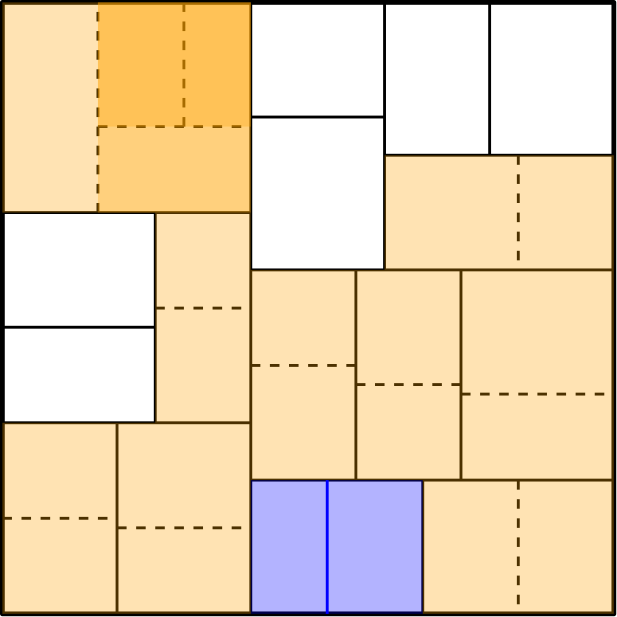
\includegraphics[width=0.45\linewidth]{figures/current.png}\hspace{2em}
    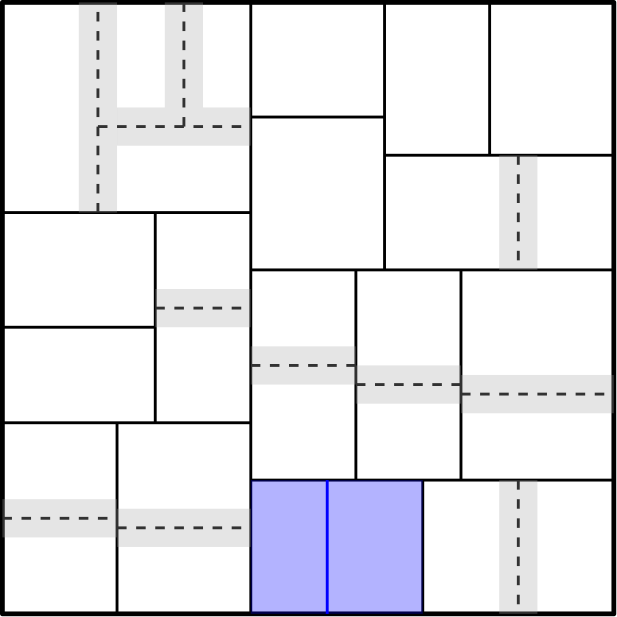
\includegraphics[width=0.45\linewidth]{figures/current2.png}
    \caption{(left) The set $\mcC_\cell$ (the cells shaded in orange with dashed lines as their divider) for a cell $\cell$ (shaded in blue), and (right) any boundary-matched point in the gray area might cause a low-net-cost execution of the extended Hungarian search procedure on $\cell$.}
    \label{fig:current}
\end{figure}
From Lemma~\ref{lemma:ratio}, for each cell $\cell'\in\mcC_\cell$ and each point $b\in \mcB_{\cell'}$,  the point $b$ is within a distance $\ell_\cell n^{-1/5} < \ell_{\cell'}\lambda$ from the divider $\Gamma_{\cell'}$, and from the construction of $\mcH$ (Lemma~\ref{lemma:margin}),
$|\mcB_{\cell'}|=O(n_{\cell'}n^{-1/5})$. Furthermore, from Lemma~\ref{lemma:ratio} and the construction of $\mcH$, each point $b\in B$ can lie inside a constant number of cells in $\mcC_\cell$; hence, $\sum_{\cell'\in\mcC_\cell}|\mcB_{\cell'}| = O(\sum_{\cell'\in\mcC_\cell}n_{\cell'} n^{-1/5}) = O(n^{4/5})$. Therefore, the total number of low-net-cost selections of $\cell$ by the extended Hungarian search procedure is $O(n^{4/5})$, as claimed. 


\subsection{Fast Search Procedures for the Geometric \texorpdfstring{$k$}{}-SP and the \texorpdfstring{$k$}{}-SPI Problems}\label{sec:hungarian_nk}


Given an instance of the geometric $k$-SP, in this section, we show that the search for the minimum net-cost augmenting path using a Hungarian search style procedure (as in the merge and extended Hungarian search procedures of our algorithm) can be done in $O(n\Phi(n)\log^3 n)$ time, where $\Phi(n)$ is the query/update time of an existing dynamic weighted nearest neighbor data structure (DWNN). 

Given a matching $M$ and dual weights $y(\cdot)$ satisfying Conditions~\eqref{eq:dualfeasibility-non-matching-time} and~\eqref{eq:dualfeasibility-matching-time}, the Hungarian search (which executes a Dijkstra's shortest path procedure) can be efficiently implemented on a complete bipartite graph using only $\tilde{O}(n)$ queries to a dynamic weighted bichromatic closest pair data structure (BCP). This search procedure grows a tree $\mathcal{T}$ by finding the cheapest cut edge under a weighted distance. See~\cite{agarwal1995vertical, ra_soda12,vaidya1989geometry} where the Hungarian search procedure that uses $O(n)$ queries to a BCP has been described. Furthermore, one can implement a BCP using a DWNN in $\tilde{O}(\Phi(n))$ time; here $\Phi(n)$ is the update/query time of the DWNN~\cite{eppstein1995dynamic}. 

In our case, the graph $\mathcal{G}_{\requests}$ is not a complete graph. However, we can easily decompose the graph into a set of $O(n)$ complete bipartite graphs as follows. Build a balanced binary search tree $T$ where the indices of requests $\{1,\ldots, n\}$ form the leaves. Let, for any node $v$, $L(v)$ denote the indices at the leaves of the left subtree of $v$ and $R(v)$ denote the indices at the leaves of the right subtree of $v$. We partition the edges as follows: At each node $v$ in $T$, we store all edges that go from the exit gates of requests with indices in $L(v)$ to the entry gates of the requests with indices in $R(V)$. See Figure~\ref{fig:cliquedec} for an example. Thus, at each node, we simply store the complete bipartite graph between points in $L(v)$ and $R(v)$. It is easy to see that any request $r_j$ participates in $O(\log n)$ cliques. 

\begin{figure}
    \centering
    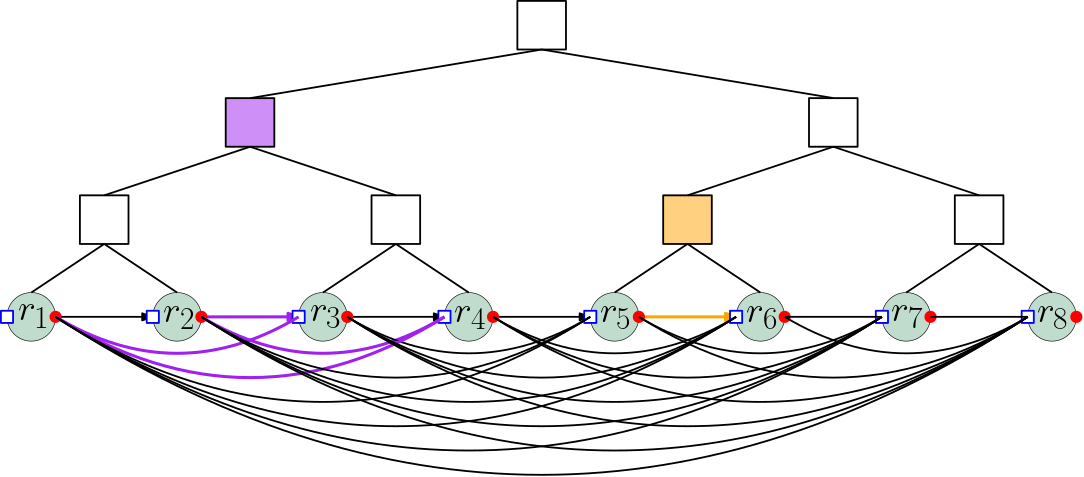
\includegraphics[width=\textwidth]{figures/ds2.png}
    \caption{The balanced binary search tree $T$ used in the construction of our dynamic weighted bichromatic closest pair data structure. The purple (resp. orange) edges in the graph are stored at the purple (resp. orange) node of $T$.}
    \label{fig:cliquedec}
\end{figure}

While executing the Hungarian search, we maintain a BCP at each node $v$ of this tree. Let $\mathcal{T}$ denote the Dijkstra's shortest path tree maintained by the Hungarian search. Our data structure stores the nodes of $L(v)$ that are currently in $\mathcal{T}$ and the nodes of $R(v)$ that are currently not in $\mathcal{T}$. The weighted bichromatic closest pair for each of these cliques is stored in a global priority queue. The query to this data structure will simply return the pair at the top of this priority queue. Adding a node $v$ to the Dijkstra's shortest path tree will trigger insertion or deletion of $v$ in the $O(\log n)$ cliques that it participates in. For each of these cliques, we update their representative pair in the global priority queue. Thus, all insertions, deletions, and queries can be done in $\tilde{O}(\Phi(n))$ time.
We obtain a fast Hungarian search by using this data structure in place of the standard dynamic weighted bichromatic closest pair data structure as used in~\cite{ra_soda12}. 

\subsection{Extension of our Sub-Quadratic to the \texorpdfstring{$k$}{-}-SPI Problem}\label{sec:kspi-extension-sub}
Our algorithm for the $k$-SP problem computes a minimum-cost $(n-k)$-matching on a graph $\mcG_\sigma$ between a point set $A$ of size $n$ and a point set $B$ of size $n$. For the $k$-SPI problem on an instance $\sigma'=\eta\sigma$, since there exists a matching on the graph $\mcG_{\requests'}$ that matches all points of $B$, one can use the same algorithm by setting $k=0$ to compute a minimum-cost $n$-matching on $\mcG_{\requests'}$. Our algorithm therefore easily extends to the $k$-SPI problem. Note that the efficiency of our algorithm only requires the existence of a matching that matches the majority of the points of $B_\cell$ in each cell $\cell$ and has a low cost (Lemma~\ref{lemma:geometric-matching}). We observe that the same property holds for the $k$-SPI problem, as the initial locations of the servers only introduce new points to the set $A_\cell$ and the number of unmatched points of $B_\cell$ in the matching constructed in Lemma~\ref{lemma:geometric-matching} remains unchanged. Therefore, our algorithm runs in $\tilde{O}(n^{9/5}\Phi(n)\log\Delta)$ time for the $k$-SPI problem as well. 









